Ebben a fejezetben szeretnék egy átfogó képet adni a helpdesk alkalmazásról.

\section{Component Diagram}


\begin{figure}[hbt] 
	\centering
	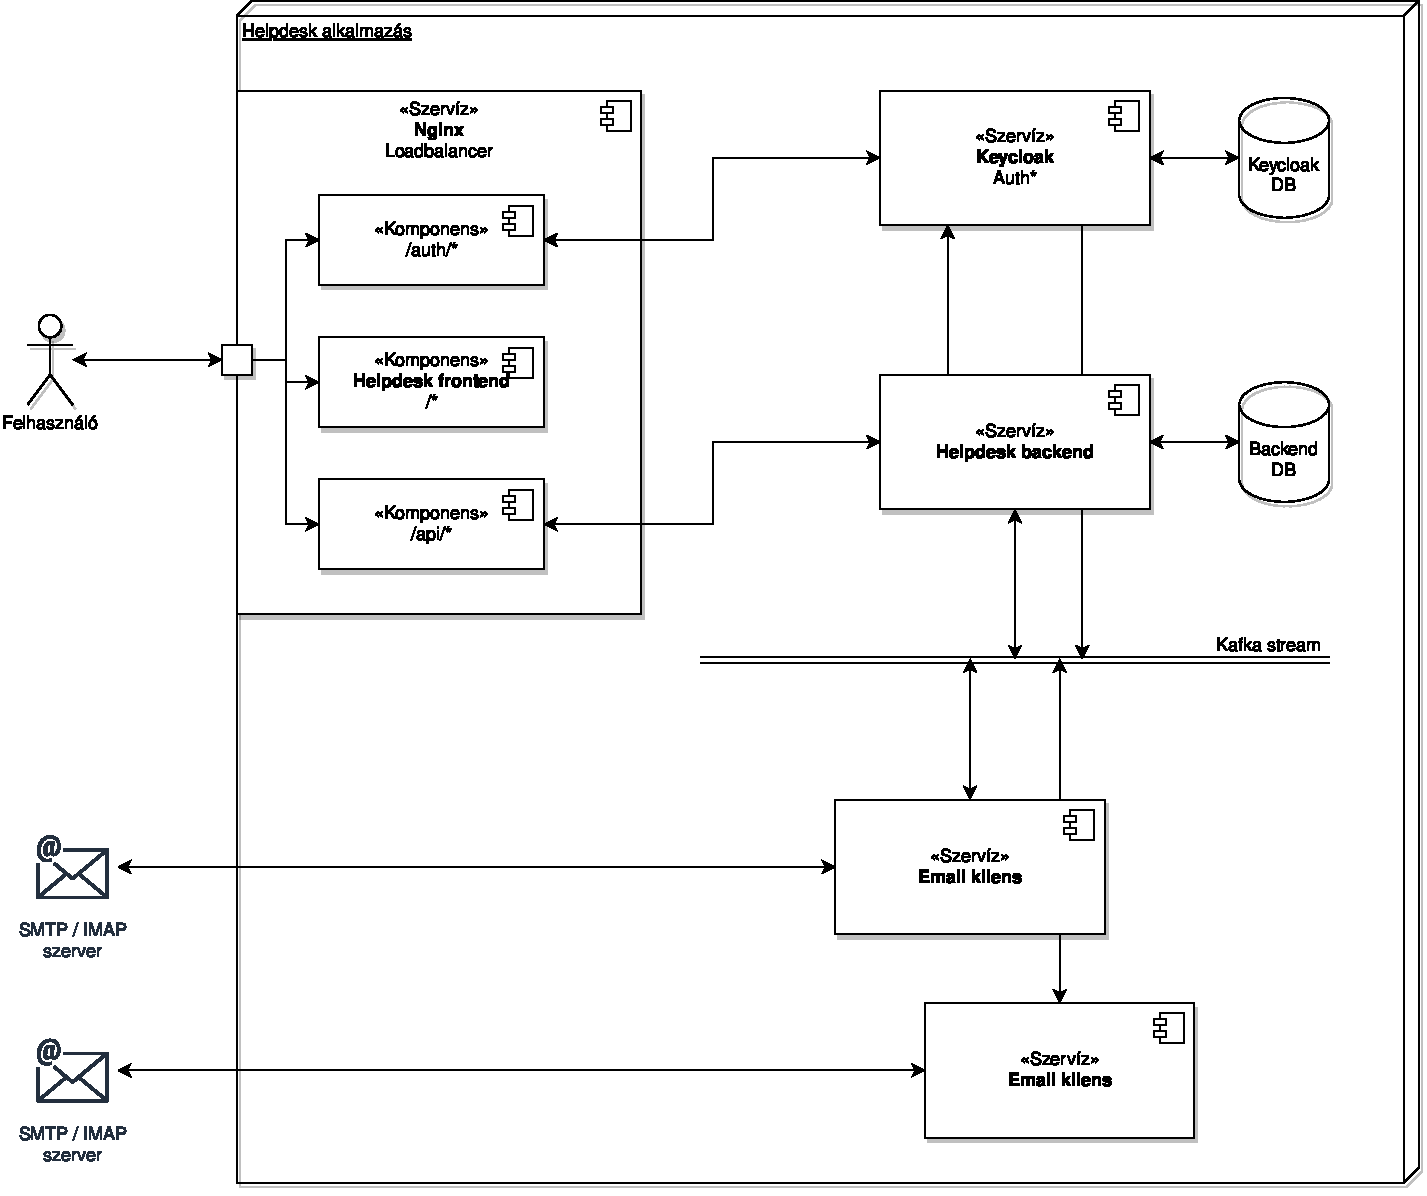
\includegraphics[width=0.85\textwidth]{komponens_diagram_drawio.pdf}
	\caption{A legfontosabb komponensek}
	\label{fig:komponens_diagram}
	\floatfoot{Forrás: saját ábra}
\end{figure}

\section{Sequence UML Diagram}
rajta legyen az összes kommunikáció majdnem mind, 
le kellene írni hogy hogyan megy a kommunikáció

\section{Adatbázis UML ábra}
audittal együtt lehet 

\section{Átfogó áttekintés az implementálás bemutatása előtt}